\section{Data Structures}
\label{sec:DataStructure}

In this section, we show how a mapper cosheaf $F:\Open(\cU)\to\Set$ can be represented as a graph and how the unnatural transformations $\phi$ and $\psi$ can be encoded as binary block matrices. We then demonstrate that the entries of the basis loss function arise from matrix multiplication.  

\begin{figure}%
    \centering
    
\includegraphics[width=0.5\linewidth]{interleave_example_F_slice_Edited.pdf}
    \caption{Example of a mapper cosheaf graph representation.
    For example, the vertices from $F(S_{\sigma_i})$ are $b$ and $c$; the edges from $F(S_{\tau_i})$ are $bd$ and $cf$.}
    \label{fig:example_slice}
\end{figure}

\subsection{Representing Mapper Cosheaves as Graphs}
\label{ssec:cosheafgraphs}

Given a mapper cosheaf $F\colon\Open(\cU) \to \Set$, we build a graph $(V_F,E_F)$ as follows. 
Recall that $K$, the one-dimensional cubical complex discretizing $\R$, consists of vertices  $\sigma_{-L},\cdots,\sigma_L$ with heights contained in the bounding box $[-L\delta,L\delta]$, along with edges ${\tau_j = (\sigma_j, \sigma_{j+1})}$. 
The graph for the mapper cosheaf $F:\Open(\cU) \to \Set$ is constructed by generating a vertex for every object in every $F(S_{\sigma_i})$, an edge for every object in every $F(S_{\tau_i})$, and connecting them using the constituent morphisms of $F$.
The resulting vertex and edge sets are
$V_F = \coprod_{i =1}^B F(S_{\sigma_i})$ and $E_F = \coprod_{i =1}^{B-1} F(S_{\tau_i})$, where the difference in index sets is a result of having an edge for every object in every $F(S_{\tau_i})$, of which there is one fewer by construction. 
The endpoints of any edge $e \in F(S_{\tau_i}) \subseteq E_F$ are found via the attaching maps: 
\[F[S_{\tau_i} \subseteq S_{\sigma_{i}}](e) \in F(S_{\sigma_i}) 
    \text{ and } 
F[S_{\tau_i} \subseteq S_{\sigma_{i+1}}](e) \in F(S_{\sigma_{i+1}}). \]
For example,  $ (c,f) \in F(S_{\tau_{i}})$ in \cref{fig:example_slice} has endpoints $c \in F(U_{\sigma_i})$ and $f \in F(U_{\sigma_{i+1}})$. 
This data is stored in a standard adjacency list, where each vertex $v \in F(U_{\sigma_i})$ stores the associated value $i$ as a representation of its height.

We next use $F$ to construct graph representations for both the functors $F^n$ and $F^{2n}$; see \cref{fig:example_all_graphs} for reference.
Since building $F^{2n}$ from $F^n$ is the same as building $F^{n}$ from $F$ up to indexing, we only describe the construction of $F^n$. 
For any $\rho \in K$, $F^n(S_{\rho}) = F(S^n_{\rho})$, and because of the cosheaf properties, this means 
\begin{equation}
\label{eq:colimit}
F^n(S_{\rho}) = \colim _{S \in S_{\rho}^n}F(S) = \colim_{S_{\rho'} \in S_{\rho}^n}F(S_{\rho'}). 
\end{equation}
If $\rho$ is a vertex $\sigma_i$, then checking indices shows that the colimit is taken over the set
\begin{equation}
\{\rho' \in K \mid S_{\rho'} \in S_{\sigma_i}^n \}
=
\{ \sigma_j \mid j \in [i-n,i+n]\} \cup \{ \tau_j \mid j \in [i-n-1,i+n]\}.
\end{equation}
The result is that $F^n(S_{\sigma_i})$ is the set of connected components of the graph induced by the vertex set 
$\coprod_{j \in [i-n,i+n]} F(S_{\sigma_j}) \subseteq V_F.$
Each connected component results in a vertex in the graph representation of $F^n$. 
This induced graph does not include any edges representing elements of $F(S_{\tau_{i-n-1}})$ or $F(S_{\tau_{i+n}})$, although these are both sets involved in the colimit of \cref{eq:colimit}.
However, since these ``half edge'' elements have maps only to $F(S_{\sigma_{i-n}})$ and $F(S_{\sigma_{i+n}})$ respectively, dropping them does not change the resulting colimit.

\begin{figure}
    \centering
    
\includegraphics[width=.8\linewidth]{interleave_example_graphs.pdf}
    \caption{Input mapper cosheaf graphs $F$ and $G$ (left) with $n$- (middle) and $2n$-smoothed versions (right).
    Vertex labels do not compare across graphs; instead, they reflect the construction methods.
    These examples correspond to the matrix examples shown in \cref{fig:boundary_matrix,fig:inclusion_matrix,fig:distance_matrix,fig:assignment_matrix}.}
    \label{fig:example_all_graphs}
\end{figure}

Similarly, for an edge $\tau_i \in K$, the colimit is taken over the set 
\begin{equation*}
\{\rho' \in K \mid S_{\rho'} \in S_{\tau_i}^n \}
=
\{ \sigma_j \mid j \in [i-n+1,i+n]\} \cup \{ \tau_j \mid j \in [i-n,i+n]\}.
\end{equation*}
and thus is the connected components of the graph induced by vertex set
\begin{equation}
\label{eq:induced_graph_for_edge_thickening}
\coprod_{j \in [i-n+1,i+n]} F(S_{\sigma_j}) \subseteq V_F.
\end{equation}
Each connected component of this graph gives an edge in the graph representation of $F^n$, 
with endpoints determined by the induced map on colimits since $S_{\tau_i}^n \subseteq S_{\sigma_i}^n$ and ${S_{\tau_i}^n \subseteq S_{\sigma_{i+1}}^n}$. 

Since connected components of a graph $(V,E)$ can be determined in $O(|V|+|E|)$ time using breadth first search, $F^n$ can be built from $F$ in $O(L \cdot (|V_F| + |E_F|))$ time.
Further, during this construction the natural transformation $F \rightarrow F^n$ can be stored at the same time; see \cref{ssec:InclusionMatrices} for more details. 
Similarly, $F^{2n}$ can be built from $F$, so getting all four additional graphs from $F$ and $G$ can be done in $O(L \cdot (|V_F| + |E_F|))$ time.

Given a graph representation of one of the functors $F$, $F^n$, or $F^{2n}$, we must determine the distance $d_{S_{\sigma_i}}(v,v')$ between any two vertices, as defined in \cref{eqn:DistanceDefinition}.
Let the mapper cosheaf $H \in \{F, F^n, F^{2n}\}$ be graphically represented by a vertex set $V$ and an edge set $E$, where each vertex $v \in V$ corresponds to a $\sigma_i$ and each edge $e \in E$ corresponds to a $\tau_i$.
For $v, v' \in H(S_{\sigma_i})$, the condition $H[S_{\sigma_i} \subseteq S_{\sigma_i}^k](v) = H[S_{\sigma_i} \subseteq S_{\sigma_i}^k](v')$ holds precisely when $v$ and $v'$ lie in the same connected component of the subgraph induced by vertices in $S_{\sigma_i}^k$.
This reduces to finding a minimum-height path between the two vertices, which can be computed by a breadth-first search (BFS) in $O(|V_F| + |E_F|)$ time.



\subsection{Representing Maps and Relationships as Block Matrices}
\label{sec:AllMatrices}

Our next task is to represent the information carried by the relevant (un)natural transformations. 
Recall that an (un)natural transformation $\eta\colon H \to H'$ consists of set maps $\eta_{S}\colon H(S) \to H'(S)$ for all $S \in \{S_\rho \mid \rho \in K\} \cup \{S^n_\rho \mid \rho \in K\}$. Let $(V_H, E_H)$ and $(V_{H'}, E_{H'})$ denote the vertex and edge sets of the graph representations of $H$ and $H'$, respectively. 
Each set map sends vertices (resp.~edges) representing elements of $H(S_{\sigma_i})$ (resp. $H(S_{\tau_i})$) to vertices (resp. edges) representing elements of $H'(S_{\sigma_i})$ (resp. $H'(S_{\tau_i})$). To encode this consistently, we impose a total order on vertices (and similarly on edges) so that if $v$ corresponds to $\sigma_i$ and $v'$ to $\sigma_j$ with $i < j$, then $v < v'$.

We store $\eta$ as a pair of block matrices $M_V \in \{0,1\}^{|V_{H'}| \times |V_H|}$ and $M_E \in \{0,1\}^{|E_{H'}| \times |E_H|}$, where an entry at $(a,a')$ is 1 iff $\eta_{S_\rho}(a) = a'$ for the appropriate $\rho \in K$. All nonzero entries therefore lie within blocks indexed by $H'(S_\rho) \times H(S_\rho)$, and each column contains exactly one $1$, with all remaining entries equal to $0$.
 
%
%
In this section, we give specifics on the matrices representing the various maps needed in the loss function computation. 

\subsubsection{Boundary Matrices}
\label{ssec:BdyMatrices}
%
    \begin{figure}[]
        \centering
        %
        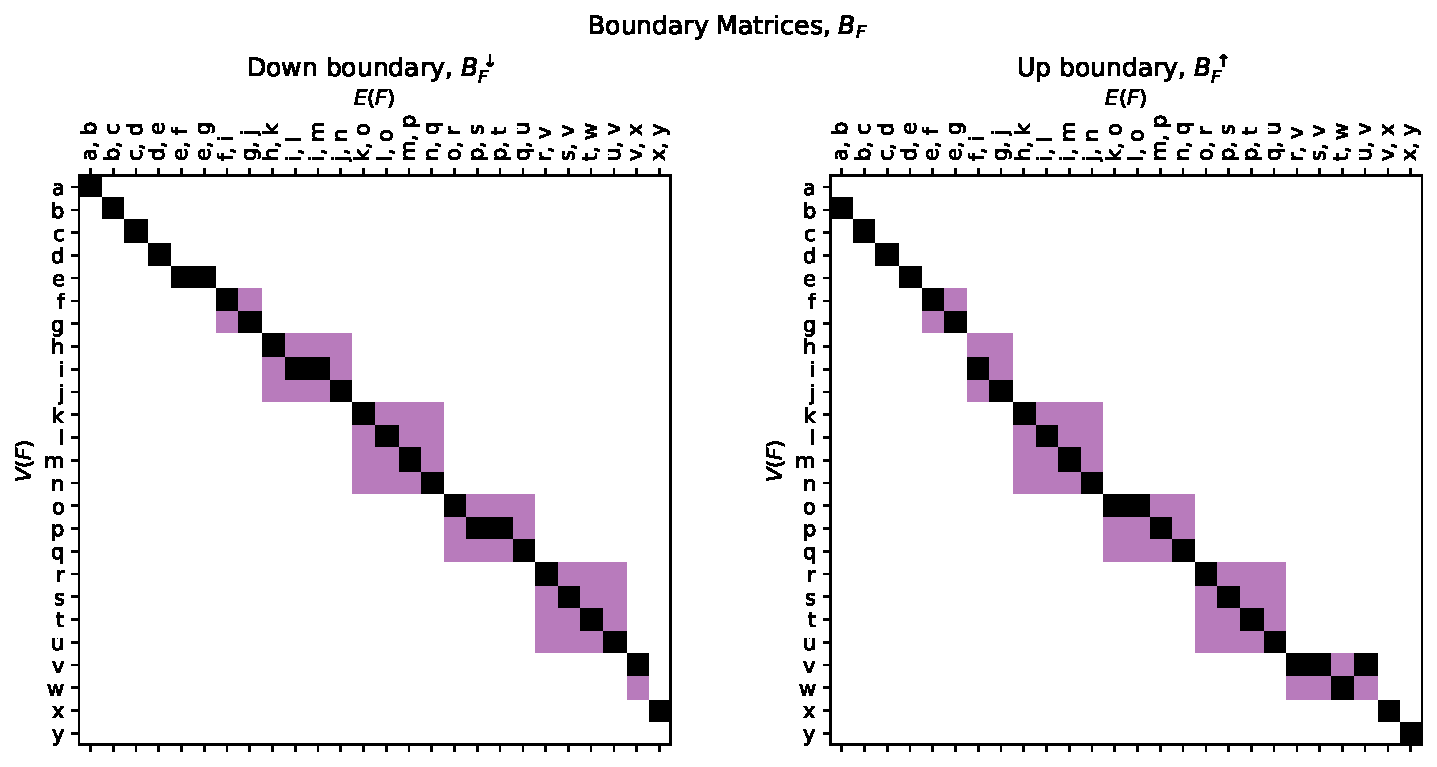
\includegraphics[width = .8\textwidth, align = c]{figures/interleave_example_boundary_matrices.pdf}
        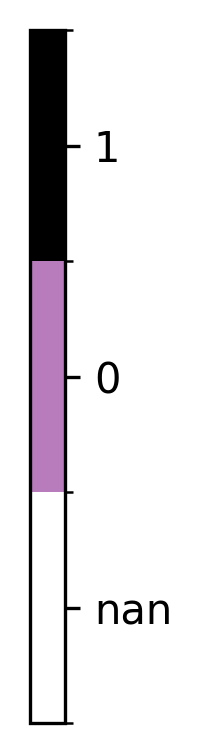
\includegraphics[width = .07\textwidth, align = c]{figures/colorbar-PurBl-binary.png}
        \caption{Example boundary matrices of the graph of $F$ shown in \cref{fig:example_all_graphs}.}
        \label{fig:boundary_matrix}
    \end{figure}
    %
The boundary matrices describe the relationship between the edges and vertices of a graph representation of a given mapper cosheaf. 
For a mapper cosheaf $H \in \{F, F^n,  G, G^n \}$, this is a matrix $B_H \in \{0,1\}^{|E_H| \times |V_H|}$, with a 1 in entry $B_H[e,v]$ iff $v$ is an endpoint of $e$. 
Unlike the other matrices we have used, this matrix has two nonzero entries in each column. However, it can be decomposed into a sum of two block matrices, each with a single nonzero entry per column, as follows. 
Let $B_H^{\uparrow} \in \{0,1\}^{|E_H| \times |V_H|}$ have a 1 in entry $B[e,v]$ iff $v$ is an endpoint of $e$ for $v \in F(\sigma_i)$ and $e \in F(\tau_{i})$; let $B_H^{\downarrow} \in \{0,1\}^{|E_H| \times |V_H|}$ have a 1 in entry $B[e,v]$ iff $v$ is an endpoint of $e$ for $v \in F(\sigma_i)$ and $e \in F(\tau_{i-1})$. 
Then $B_H = B_H^{\uparrow} + B_H^{\downarrow}$; see \cref{fig:boundary_matrix} for an example. 
In this case, we will have eight matrices to work with, which we denote by 
$B_F^{\uparrow}$, $B_F^{\downarrow}$, 
$B_{F^n}^{\uparrow}$,  $B_{F^n}^{\downarrow}$,  
$B_G^{\uparrow}$, $B_G^{\downarrow}$, 
$B_{G^n}^{\uparrow}$, and $B_{G^n}^{\downarrow}$.
We do not compute the boundary matrices for either $F^{2n}$ or ${G}^{2n}$ since, as can be seen in \cref{tab:theList}, these matrices are never used.
Because these are simply matrix encodings of the adjacency information of the relevant graphs, they can be constructed in $O(V_{\max} \cdot E_{\max})$ time, where $V_{\max} = \max\{|V_H| \mid H \in F, F^n,  G, G^n  \}$ and $E_{\max} = \max\{|E_H| \mid H \in F, F^n,  G, G^n  \}$.


    %
    %
    %
    %

    %
    %
    %
    %
    %
    %
    %
    %
    %
    %

  %
\subsubsection{Inclusion Matrices} 
\label{ssec:InclusionMatrices}
%
    \begin{figure}[!htb]
        \centering
        %
        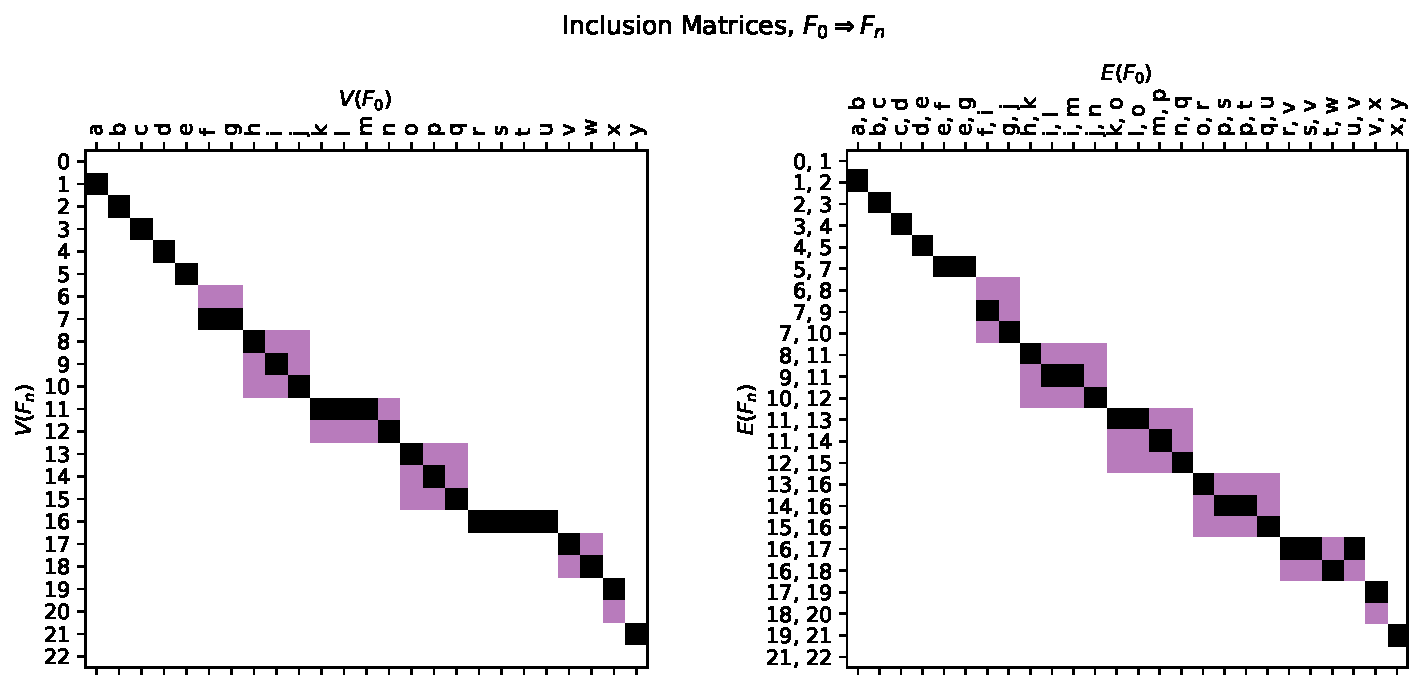
\includegraphics[width = .8\linewidth, align = c]{figures/interleave_example_inclusion_matrices.pdf}
        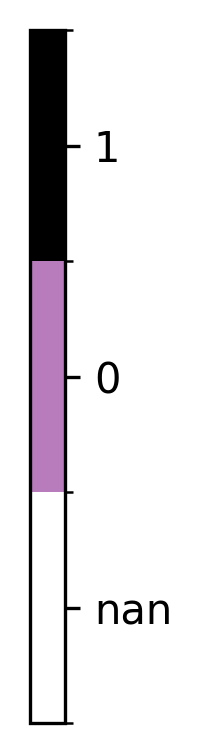
\includegraphics[width = .07\textwidth, align = c]{figures/colorbar-PurBl-binary.png}
        \caption{Inclusion matrices $I_F^V$ (left) and $I_F^E$ (right) representing $F \Rightarrow F_n$ from \cref{fig:example_all_graphs}.}
        \label{fig:inclusion_matrix}
    \end{figure}

The inclusion matrices represent the natural transformations $F \Rightarrow F_n \Rightarrow F_{2n}$ and $G  \Rightarrow G_n  \Rightarrow G_{2n}$.
Focusing on the first of these, $F \Rightarrow F^n$, the component morphisms take a vertex $v \in F(S_{\sigma_i})$ to the vertex $v' \in F^n(S_{\sigma_i})$ representing the connected component containing $v'$. 
The edge maps are determined similarly. 
    Thus the vertex inclusion matrix is written as $I_F^V \in \{0, 1 \}^{|V_{F^n}| \times |V_{F}|}$ with a 1 in entry $I_F[v',v]$ if $v$ is in the connected component represented by $v'$.
    A similar matrix is built for the edges, $I_F^E \in \{0, 1 \}^{|E_{F^n}| \times |E_{F}|}$. 
    The result is that each inclusion natural transformation is given by a pair of matrices, so from this construction we have the matrices $I_F^V$, $I_F^E$, $I_{F^n}^V$, $I_{F^n}^E$, $I_G^V$, $I_G^E$, $I_{G^n}^V$, $I_{G^n}^E$; see \cref{fig:inclusion_matrix} for an example. 
These matrices satisfy the block decomposition and have exactly one nonzero entry in each column. They also have the useful property that the inclusion functor from a graph to its $2n$-smoothing can be computed via matrix multiplication; for example, the induced map on vertices for $F \Rightarrow F_{2n}$ is given by $I_{F^n}^V I_F^V$. Moreover, since they track representatives of objects in the $n$-smoothed connected components, these matrices can be constructed alongside the smoothed graphs with only constant overhead. 

    

    

    
    
    %
    %
    %
    %
    %

    %


%
\subsubsection{Distance Matrices}
%
\label{ssec:DistanceMatrices}
     \begin{figure}[!htb]
       \centering
        %
        %
        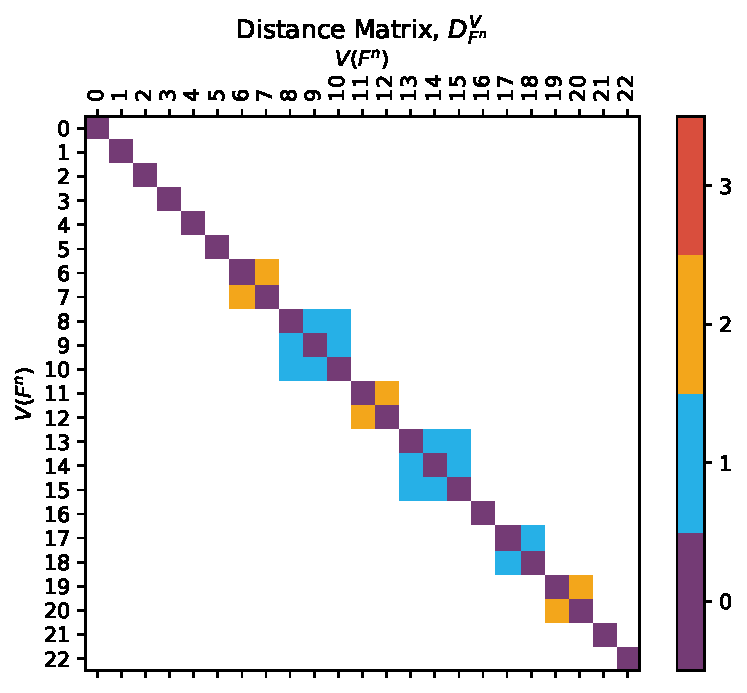
\includegraphics[width = .4\linewidth, align = c]{figures/interleave_example_distance_matrix.pdf}
        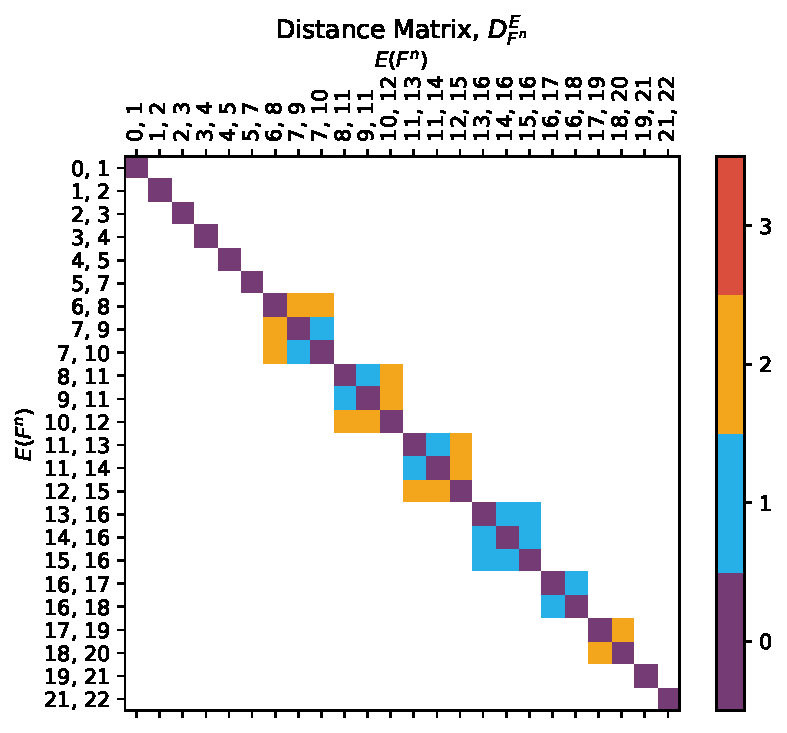
\includegraphics[width = .4\linewidth, align = c]{figures/interleave_example_distance_matrix_edges.pdf}
        \caption{Distance matrix example for $F^n$ from \cref{fig:example_all_graphs}.}
        \label{fig:distance_matrix}
    \end{figure}
The distance matrices encode the distance from \cref{eqn:DistanceDefinition}. 
In particular, for vertices $v,w \in F(S_\rho)$, we seek the minimum $k$ such that they map to the same object in $F(S_\rho^k)$. 
Equivalently, this is the minimum $k$ where $v$ and $w$ are in the same connected component of the subgraph induced by the vertex set $\coprod_{S_{\sigma_i} \subseteq S_\rho^k} F(S_{\sigma_i})$.
For example, in the graph of $F^n$ from \cref{fig:example_all_graphs}, vertices $11$ and $12$, both at level $\sigma_9$, are not in the same connected component until $k=2$ using the path through vertex $7$ below. 
Similarly, edges $(12,15)$ and $(11,14)$ have distance 2 via the path through vertex $7$.


This distance is stored as a pair of matrices $D_F^V \in \{0,1\}^{|V(F)|^2}$ and $D_F^E\in \{0,1\}^{|E(F)|^2}$. 
For the vertices, $D_F^V[u,v] = d_{S_{\sigma_i}}(u,v)$ if $u,v \in F(S_{\sigma_i}) \subset V_F$, and 0 otherwise; $D_F^E$ is defined similarly for the elements of $F(S_{\tau_i})$.
These matrices inherit the block structure determined by the mapper cosheaf heights.
See \cref{fig:distance_matrix} for examples corresponding to $F^n$ from \cref{fig:example_all_graphs}. 
In total, we have 12 distance matrices, two each for the six input matrices. 
However, as noted in \cref{tab:theList}, only the eight for $F^n$, $F^{2n}$, $G^n$, and $G^{2n}$ need to be calculated. 

We now compute these distance matrices from the graph representations.
For each level $i \in [-L,L]$, we construct the block for $\sigma_i$ and $\tau_i$ in $D_F^V$  and $D_F^E$ respectively.
In the vertex case, we build a union-find data structure by adding the edges in order of increasing thickening. 
Recall (and see \cref{fig:PosetNotation} for notation reminder) that the elements of $F(S^k_{\sigma_i})$ correspond to the subgraph induced by the vertices in $\coprod _{j \in [i-n,i+n]} F(S_{\sigma_j})$, which includes the edges in $\coprod_{j \in [i-k, i+k-1]}F(S_{\tau_j})$. 
Therefore, for $k=1$, we add all edges corresponding to $\tau_{i-1}$ and $\tau_i$. Note that the edges for $\tau_{i-2}$ and $\tau_{i+1}$ are irrelevant here, as they do not involve any vertices in $S_{\sigma_j}^1$ and thus cannot affect connectivity. We then check whether any vertices in $F(S_{\sigma_i}^1)$ lie in the same connected component. For each pair $u$ and $v$ that do, we set $D_F^V[u,v] = 1$.
Then for $k=2$, we add the edges for $\tau_{i-2}$ and $\tau_{i+2}$, and repeat the same check for pairs that are not already in the same connected component at $k=1$, setting these distances to 2 if they are now in the same component. 
We continue until all pair distances are determined. 

A similar sweep for each level is used to construct $D_F^E$, with the difference being that the edges added at step $k$ are those from $F(\tau_{i-k+1}, \tau_{i+k-1})$. 
We have $V_{\max}$ entries in our union-find data structure, so amortized time per operation is $O(\alpha(V_{\max}))$, with a total of $E_{\max}$ operations.
Thus, since the union-find structure is built at each level, the pair of matrices for a given graph takes time $O(L\cdot E_{\max} \cdot \alpha(V_{\max}))$, where $\alpha(\cdot)$ is the inverse Ackermann function. 



\subsubsection{Assignment Matrices}
%
\begin{figure}[!ht]
        \centering
        
\includegraphics[width=.8\linewidth, align = c]{interleave_example_phi.pdf}
        
\includegraphics[width = .07\textwidth, align = c]{colorbar-PurBl-binary.png}
        \vspace{-4mm}
        \caption{Matrices for an input unnatural transformation $\phi$ of the example graphs in \cref{fig:example_all_graphs}. }
        \label{fig:assignment_matrix}
        %
\end{figure}
%
%

%

%

To solve for assignment choices, we record them as matrices. Given an $n$-assignment $\phi$ and $\psi$, we first restrict each map to $S_\rho$ and $S_\rho^n$, and then separate these restrictions according to whether $\rho$ is a vertex ($\rho = \sigma_i$) or an edge ($\rho = \tau_i$). The four resulting matrices for $\phi$ (with analogous matrices for $\psi$) are denoted as 
\begin{equation*}
    \begin{matrix}
    M_\phi^V \in \{0,1\}^{|V(G^n)| \times |V(F)|}, & 
    M_{\phi_n}^V \in \{0,1\}^{|V(G^{2n})| \times |V(F^n)|}, \\ 
    M_\phi^E \in \{0,1\}^{|E(G^n)| \times |E(F)|}, &
    M_{\phi_n}^E \in \{0,1\}^{|E(G^{2n})| \times |E(F^n)|}. 
    \end{matrix}
    \end{equation*}
As with the other matrices, these are block matrices aligned with the $\sigma_i$ and $\tau_i$ indices, each containing exactly one 1 per column. The matrix $M_\phi^V$ satisfies $M_\phi^V[u,v] = 1$ iff $\phi_{S_{\sigma_i}}(u) = v$ for $u \in F(S_{\sigma_i})$ and $v \in G(S_{\sigma_i}^n)$. An example is shown in \cref{fig:assignment_matrix}, where $\phi$ is randomly generated so that each column contains a single 1; in this case, the associated parallelogram diagram fails to commute, indicating that $\phi$ is not a natural transformation. In our ILP formulation, we search over such assignment matrices to identify choices of $\phi$ and $\psi$ that minimize the loss. We need only initialize empty matrices in the setup.




%
\subsection[]{Binary Decision and Loss Computation for Fixed $\phi$ and $\psi$}

%
\begin{table}[]
    \centering
\begin{tabular}{|r|p{1cm}|c|c|c|}
\hline 
&   \centering{\textbf{Loss Term}}   & \textbf{Diagram} & \textbf{Matrix Multiplication} & \textbf{Eval.}\\ \hline \hline
\multirow{2}{*}{\rotatebox[origin=r]{90}{$\substack{\text{Edge-Vertex \hfill}\\\text{Parallelogram \hfill}}$}}
& $\Lpl^{S_\tau, S_\sigma}$
& 
    $
    \begin{tikzcd}[scale cd = .7]
    F(S_\tau)  
        \ar[r, "{F[\subseteq ]}"] 
        \ar[dr, "\varphi_{S_\tau}"']
    & F(S_\sigma)
        \ar[dr, "\varphi_{ S_\sigma}"]
    & \\
    & G^n(S_\tau) 
        \ar[r, "{G[\subseteq ]}"'] 
    & G^n(S_\sigma)  
    \end{tikzcd}
    $
&
    \parbox{4.5cm}{
\centering
        $D_{G^n}^V \left(M_{\phi}^V \cdot B_F^{\uparrow} - B_{G^n}^{\uparrow} \cdot M_{\phi}^E\right)$\\
        $D_{G^n}^V \left(M_{\phi}^V \cdot B_F^{\downarrow} - B_{G^n}^{\downarrow} \cdot M_{\phi}^E\right)$
   }
%
& \multirow{4}{*}[-11.5ex]{$\max(A)$}
\\
\cline{2-4}
& $\Lpr^{S_\tau, S_\sigma}$
&
    $
    \begin{tikzcd}[scale cd = .7]
    & F^n(S_\tau) 
        \ar[r, "{F[\subseteq ]}"] 
    & F^n(S_\sigma)  
    \\
    G(S_\tau)  
        \ar[r, "{G[\subseteq ]}"'] 
        \ar[ur, "\psi_{S_\tau}"]
    & G(S_\sigma)
        \ar[ur, "\psi_{ S_\sigma}"']
    \end{tikzcd}
    $
&
\parbox{4.5cm}{
\centering
    $D_{F^n}^V \left(M_{\psi}^V \cdot B_G^{\uparrow} - B_{F^n}^{\uparrow} \cdot M_{\psi}^E\right)$\\
    $D_{F^n}^V \left(M_{\psi}^V \cdot B_G^{\downarrow} - B_{F^n}^{\downarrow} \cdot M_{\psi}^E\right)$
}
& 
\\
\cline{2-4}
\multirow{2}{*}{\rotatebox[origin=r]{90}{$\substack{\text{Thickening \hfill}\\\text{Parallelogram \hfill}}$}}
& $\Lpl^{S_\rho, S_\rho^n}$
& 
    $
    \begin{tikzcd}[scale cd = .7]
    F(S_\rho)  
        \ar[r, "{F[\subseteq ]}"] 
        \ar[dr, "\varphi_{S_\rho}"']
    & F^n(S_\rho)
        \ar[dr, "\varphi_{ S_\rho^n}"]
    & \\
    & G^n(S_\rho) 
        \ar[r, "{G[\subseteq ]}"'] 
    & G^{2n}(S_\rho)  
    \end{tikzcd}
    $
&
\parbox{4.5cm}{
\centering
    $D_{G^{2n}}^V \left(M_{\phi^n}^V \cdot I_F^V - I_{G^n}^V \cdot M_{\phi}^V\right)$\\
    $D_{G^{2n}}^E \left(M_{\phi^n}^E \cdot I_F^E - I_{G^n}^E \cdot M_{\phi}^E\right)$
}
&
\\
\cline{2-4}
& $\Lpr^{S_\rho, S_\rho^n}$
&
    $
    \begin{tikzcd}[scale cd = .7]
    & F^n(S_\rho) 
        \ar[r, "{F[\subseteq ]}"] 
    & F^{2n}(S_\rho)  
    \\
    G(S_\rho)  
        \ar[r, "{G[\subseteq ]}"'] 
        \ar[ur, "\psi_{S_\rho}"]
    & G(S_\rho^n)
        \ar[ur, "\psi_{ S_\rho^n}"']
    \end{tikzcd}
    $
&
\parbox{4.5cm}{
\centering
    $D_{F^{2n}}^V \left(M_{\psi^n}^V \cdot I_G^V - I_{F^n}^V \cdot M_{\psi}^V\right)$\\
    $D_{F^{2n}}^E \left(M_{\psi^n}^E \cdot I_G^E - I_{F^n}^E \cdot M_{\psi}^E\right)$
}
& \parbox{3.5cm}{
\centering}
\\
\hline
\multirow{2}{*}[-0.4ex]{\rotatebox[origin=r]{90}{Triangle \hfill}}
& $\Ltd^{S_\rho}$
&
    $
    \begin{tikzcd}[scale cd = .7]
        F(S_\rho) 
            \ar[rr, "{F[ \subseteq ]}"]   
            \ar[dr, "\phi_{S_\rho}"'] 
            & & F^{2n}(S_\rho)
        \\
        & G^n(S_\rho)\ar[ur, "\psi_{S^n_\rho}"']  & 
    \end{tikzcd}
    $
&
    \parbox{4.5cm}{
\centering
    $D_{F^{2n}}^V \left(I_{F^n}^V \cdot I_F^V - M_{\psi^n}^V\cdot M_{\phi}^V \right)$\\
    $D_{F^{2n}}^E \left(I_{F^n}^E \cdot I_F^E - M_{\psi^n}^E\cdot M_{\phi}^E \right)$
    }
    %
    & \multirow{2}{*}[-3.5ex]{\vspace{\fill}$\left\lceil \tfrac{1}{2}\max(A)\right\rceil$}
\\
\cline{2-4}
& $\Ltu^{S_\rho}$
&
    $
    \begin{tikzcd}[scale cd = .7]
        & F^n(S_\rho)\ar[dr, "\phi_{S^n_\rho}"]  & 
        \\
        G(S_\rho) 
            \ar[rr, "{G[ \subseteq ]}"']   
            \ar[ur, "\psi_{S_\rho}"] 
            & & G^{2n}(S_\rho)
    \end{tikzcd}
    $
&
   \parbox{4.5cm}{
\centering
    $D_{G^{2n}}^V \left(I_{G^n}^V \cdot I_G^V - M_{\phi^n}^V\cdot M_{\psi}^V \right)$\\
    $D_{G^{2n}}^E \left(I_{G^n}^E \cdot I_G^E - M_{\phi^n}^E\cdot M_{\psi}^E \right)$
    }
& 
\\
\hline
\end{tabular}
%
\caption{The list of loss terms, relevant diagram, and matrix multiplications. The final column shows the result from the final matrix, where the multiplied matrix is denoted $A$: either the maximum entry in the multiplied matrix, or the ceiling of half the maximum.} 
\label{tab:theList}
\end{table}

%

In this section, we use the matrices introduced above to begin addressing \cref{prob:BinaryDecision} and \cref{prob:LossComputation}. 
Throughout, we use the notation $\max(A)$ to denote the maximum entry in the matrix $A$.
For the binary decision problem, we focus on the version of the problem for a fixed assignment as follows.
We give the answers for these two problems by showing the matrix multiplications needed to check the commutativity of all diagrams (for \cref{prob:BinaryDecisionFixedAssignment}); or for computing each term in the loss function (for \cref{prob:LossComputationFixedAssignment}). 
In order to determine if $\phi,\psi$ is an interleaving and thus answer \cref{prob:BinaryDecisionFixedAssignment}, we need to check commutativity of all the diagrams in the second column of \cref{tab:theList}. 
Due to symmetry, we limit our discussion to checking commutativity of the diagrams  $\Parallelograml_\phi(S_\tau,S_\sigma)$, $\Parallelograml_\phi(S_\rho,S_\rho^n)$, and $\triangled(S_\rho)$. 
For \cref{prob:LossComputationFixedAssignment}, we need to show how  each term in   
\begin{equation*}
L_B(\phi,\psi) = \max_{ \substack{\sigma < \tau \in K \\ \rho \in K}}
\left\{
\Lpl^{S_\tau, S_\sigma}, \Lpr^{S_\tau, S_\sigma},
\Lpl^{S_\rho, S_\rho^n}, \Lpr^{S_\rho, S_\rho^n},
\Ltu^{S_\rho}, \Ltd^{S_\rho}
\right\}
\end{equation*}
corresponds to matrix multiplication in this setting.
Again, due to symmetry, we limit our discussion to $\Lpl^{S_\tau, S_\sigma}, \Lpl^{S_\rho, S_\rho^n}$, and $\Ltd^{S_\rho}$; the full list can be found in \cref{tab:theList}.
%
For a matrix $A$, we write $\max(A) \coloneqq \max_{i,j} A_{ij}$  to denote the maximum entry of $A$.


%
%
%
%
%
%
%
%
%
%

%
\subsubsection{Parallelograms}
 First, consider the diagram $\Parallelograml_\phi(S_\tau,S_\sigma)$ given by 
  \begin{equation*}
    \begin{tikzcd}
    F(S_{\tau})  
        \ar[r, "{F[\subseteq ]}"] 
        \ar[dr, "\varphi_{S_\tau}"']
    & F(S_\sigma)
        \ar[dr, "\varphi_{ S_\sigma}"]
    & \\
    & G^n(S_\tau) 
        \ar[r, "{G[\subseteq ]}"'] 
    & G^n(S_\sigma)  
    \end{tikzcd}
 \end{equation*}
 In our previous notation, we have that $\sigma_i$ is the lower vertex of $\tau_i$, and $\sigma_{i+1}$ is the upper vertex. 
 
\begin{figure}
    \centering
    
\includegraphics[width=\linewidth]{interleave_example_parallelogram_edge_vert_mult.pdf}
    \caption{Example of the matrix multiplications used to to compute the loss function for the $\Lpl(S_\tau,S_\sigma)$ case (\cref{lem:matrix_entries_edge_vert_down_binary,lem:matrix_entries_edge_vert_down}). 
    White entries in the first three matrices are outside of the block structure, and can be assumed to be 0 although they are stored as \texttt{NaN}. 
    The loss in this case is the maximum absolute entry in the last matrix.
    %
    } 
    \label{fig:multiplicationExamples_Parallelogram}
\end{figure}

\begin{lemma}
\label{lem:matrix_entries_edge_vert_down_binary}
The diagrams $\{\Parallelograml_\phi(S_{\tau_i},S_{\sigma_i})\}_i$ all commute if and only if 
\begin{equation*}
M_{\phi}^V \cdot B_F^{\downarrow} - B_{G^n}^{\downarrow} \cdot M_{\phi}^E = 0.
\end{equation*}
The diagrams $\{\Parallelograml_\phi(S_{\tau_{i+1}},S_{\sigma_i})\}_i$ all commute if and only if 
\begin{equation*}
M_{\phi}^V \cdot B_F^{\uparrow} - B_{G^n}^{\uparrow} \cdot M_{\phi}^E = 0.
\end{equation*}
\end{lemma} 

See \cref{fig:multiplicationExamples_Parallelogram} for examples of the matrices from the statement.

\begin{proof}
We will focus on proving the first statement since the methodology is the same for the second. 
Fix an $i$.  
Throughout the proof we write $\sigma = \sigma_i$ and $\tau = \tau_i$. 
We are checking whether the images landing in the bottom right of the diagram
 \begin{equation*}
    \begin{tikzcd}
    F(S_{\tau})  
        \ar[r, "{F[\subseteq ]}"] 
        \ar[dr, "\varphi_{S_\tau}"']
    & F(S_\sigma)
        \ar[dr, "\varphi_{ S_\sigma}"]
    & \\
    & G^n(S_\tau) 
        \ar[r, "{G[\subseteq ]}"'] 
    & G^n(S_\sigma)  
    \end{tikzcd}
 \end{equation*}
 are the same. 
 Fix any element $e \in F(S_{\tau})$. 
 If it has lower vertex $v \in F(S_\sigma)$ with $\phi_{S_\sigma}(v) = v'$, then the composition along the top of the diagram sends $e \mapsto v'$. 
 This means that the column for $e$ in $M_{\phi}^V \cdot B_F^{\downarrow}$ has exactly one 1 in the row corresponding to $v'$. 
If $\phi_{S_\tau}(e) = e' \in G^n(S_\tau)$ which has lower vertex $v''$, then the composition along the bottom of the diagram sends $e \mapsto v''$. 
Similarly, the column for $e$ in $B_{G^n}^{\downarrow} \cdot M_{\phi}^E$ has exactly one 1 in the row corresponding to $v''$. 
Writing $A\coloneqq M_{\phi}^V \cdot B_F^{\downarrow} - B_{G^n}^{\downarrow} \cdot M_{\phi}^E$, the column for $e$ in $A$ is entirely 0 if and only if $v' = v''$. 
This means that the matrix $A$ is entirely 0 iff $G[\subseteq]\circ \phi_{S_\tau}(e) =  \phi_{S_\sigma}\circ F[\subseteq](e)$ for all $e \in F(S_\tau)$ which is the definition of the diagram commuting. 
\end{proof}
 

We next use the above construction to determine  $\Lpl^{S_\tau, S_\sigma}$.


 \begin{lemma}
\label{lem:matrix_entries_edge_vert_down}
    %
    $\max_{i} \Lpl^{S_{\tau_i}, S_{\sigma_i}} = \max \left( D_{G^n}^V \left(M_{\phi}^V \cdot B_F^{\downarrow} - B_{G^n}^{\downarrow} \cdot M_{\phi}^E\right) \right)$
\end{lemma}

\begin{proof} 
%
Fix an $i$ and again write $\sigma = \sigma_i$ and $\tau = \tau_i$. 
Following the notation of the proof of \cref{lem:matrix_entries_edge_vert_down_binary}, given an $e \in F(S_{\tau})$ we write $v' = \phi_{S_\sigma}\circ F[\subseteq](e)$ and $v'' = G[\subseteq]\circ \phi_{S_\tau}(e) $. 
From the discussion above, this means that the column for $e$ in $M_{\phi}^V \cdot B_F^{\downarrow}$ has exactly one 1 in the row corresponding to $v'$ and the column for $e$ in $B_{G^n}^{\downarrow} \cdot M_{\phi}^E$ has exactly one 1 in the row corresponding to $v''$. 
This means that, writing $A\coloneqq M_{\phi}^V \cdot B_F^{\downarrow} - B_{G^n}^{\downarrow} \cdot M_{\phi}^E$, the column for $e$ in $A$ is either entirely 0 if $v' = v''$ or its only non-zero entries are $A[v',e] = 1$ and $A[v'',e] = -1$. 

We can  left-multiply the matrix $A$ by the distance matrix $D\coloneqq D_{G^{n}}^V$.
Clearly, if $v' = v''$ and thus the column in $A$ for $e$ is 0, the column for $e$ in $D \cdot A$ is 0. 
If $v' \neq v''$, the entries for the column $e$ are 
\begin{equation*}
    (D \cdot A)[u,e] = 
    \begin{cases}
        -d(v',v'') & \text{if } u = v'\\
        d(v',v'') & \text{if } u = v'' \\
        d(u,v') - d(u,v'') & \text{else}
    \end{cases}
\end{equation*}
where $d$ denotes the distance function $d^G_{S^n_\sigma}$. 
However, since $d(u,v') - d(u,v'') \leq d(v',v'')$ by the triangle inequality, the maximum entry in the column occurs at entry $[v'', e]$. 
This means that $\Lpl^{S_{\tau_i}, S_{\sigma_i}}$ is the maximum in the columns corresponding to $e \in F(S_{\tau_i})$. 
Further, the maximum of $\Lpl^{S_{\tau_i}, S_{\sigma_i}}$ over all $i$ is the maximum over all columns, so the lemma follows. 
\end{proof} 

A similar argument gives the following lemma for the upper vertex rather than the lower vertex of $\tau_i$. 
\begin{lemma}
\label{lem:matrix_entries_edge_vert_up}
    $\max_{i} \Lpl^{S_{\tau_i}, S_{\sigma_{i+1}}} = \max \left( D_{G^n}^V \left(M_{\phi}^V \cdot B_F^{\uparrow} - B_{G^n}^{\uparrow} \cdot M_{\phi}^E\right) \right)$
\end{lemma}

%
%
%

Next we consider the thickening matrix type, $\Lpl^{S_\rho, S_\rho^n}$. In this notation, $\rho$ can be either an edge $\tau_i$ or a vertex $\sigma_i$; we start with the vertex case $\rho = \sigma_i$. 

\begin{lemma}
\label{lem:matrix_entries_parallel_thickening}
The diagrams $\{\Parallelograml_\phi(S_{\sigma_i},S_{\sigma_i}^n)\}_i$ all commute if and only if 
\begin{equation*}
M_{\phi^n}^V \cdot I_F^V - I_{G^n}^V \cdot M_{\phi}^V= 0.
\end{equation*}
The loss is determined by
\begin{equation*}
\max_{i} \Lpl^{S_{\sigma_{i}},S_{\sigma_{i}}^n} = \max \left(D_{G^n}^V \left(M_{\phi^n}^V \cdot I_F^V - I_{G^n}^V \cdot M_{\phi}^V\right) \right).
\end{equation*}
\end{lemma}

\begin{proof} %
We are looking for the distance between images in the bottom right of 
\begin{equation*}
\begin{tikzcd}
F(S_{\sigma_i})  
    \ar[r, "{F[\subseteq ]}"] 
    \ar[dr, "{\varphi_{S_{\sigma_i}}}"']
& F^n(S_{\sigma_i})
    \ar[dr, "{\varphi_{ S_{\sigma_i}^n}}"]
& \\
& G^n(S_{\sigma_i}) 
    \ar[r, "{G[\subseteq ]}"'] 
& G^{2n}(S_{\sigma_i})  .
\end{tikzcd}
\end{equation*} 
By a similar argument to \cref{lem:matrix_entries_edge_vert_down}, if we have elements in the diagram of the form
\begin{equation*}
\begin{tikzcd}
v \ar[r, mapsto] \ar[dr, mapsto] & v' \ar[dr, mapsto]\\ 
& \substack{\\w} \ar[r, mapsto, shift right] & \substack{w'\\w''}
\end{tikzcd}
\end{equation*}
then column corresponding to $v$ in  $A = M_{\phi}^V \cdot B_F^{\downarrow} - B_{G^n}^{\downarrow} \cdot M_{\phi}^E$ will be 0 iff $w'=w''$, so the diagrams all commute iff $A = 0$. 
Likewise the column for $v$ in  
$D_{G^n}^V \left(M_{\phi}^V \cdot B_F^{\downarrow} - B_{G^n}^{\downarrow} \cdot M_{\phi}^E\right)$ 
will be entirely 0 if $w' = w''$ and will have maximum entry $d^{G^{2n}}_{S_{\sigma_i}}(w', w'')$ in the entry $[w'',v]$ otherwise. 
The lemma follows.
%
%
%
%
\end{proof}

Again, a parallel argument shows the edge thickening diagram contribution. 

\begin{lemma}
\label{lem:parallelogramcommute}
The diagrams $\{\Parallelograml_\phi(S_{\tau},S_{\tau}^n)\}_i$ all commute if and only if 
\begin{equation*}
M_{\phi^n}^E \cdot I_F^V - I_{G^n}^E \cdot M_{\phi}^E= 0.
\end{equation*}
The loss is determined by
\begin{equation*}
\max_{i} \Lpl^{S_{\tau_{i}},S_{\tau_{i}}^n} = \max \left(D_{G^n}^E \left(M_{\phi^n}^E \cdot I_F^V - I_{G^n}^E \cdot M_{\phi}^E\right) \right).
\end{equation*}
\end{lemma}

%
\subsubsection{Triangles}
The last type of loss contribution is that of the triangle diagrams, and the representation of the commutativity of the diagram is similar to the two previous examples. 
However, the one difference in this case is that the resulting loss function is the ceiling of half of the maximum, so in this case we have the following. 

\begin{lemma}
\label{lem:trianglecommute}    
The diagrams $\{\triangled_\phi(S_{\sigma_i})\}_i$ all commute if and only if 
\begin{equation*}
I_{F^n}^V \cdot I_F^V - M_{\psi^n}^V\cdot M_{\phi}^V= 0.
\end{equation*}
The diagrams  $\{\triangleu_\phi(S_{\tau_i})\}_i$ all commute if and only if 
\begin{equation*}
I_{F^n}^E \cdot I_F^E - M_{\psi^n}^E\cdot M_{\phi}^E = 0.
\end{equation*}
The loss in each case is determined by
\begin{align*}
%
%
\max_{i} \Ltd^{S_{\sigma_{i}},} &= \left\lceil\frac{1}{2}\max\left(D_{F^{2n}}^V \left(I_{F^n}^V \cdot I_F^V - M_{\psi^n}^V\cdot M_{\phi}^V \right) \right) \right\rceil,\\
\max_{i} \Ltd^{S_{\tau_{i}},} &= \left\lceil\frac{1}{2}\max\left(D_{F^{2n}}^V \left(I_{F^n}^V \cdot I_F^V - M_{\psi^n}^V\cdot M_{\phi}^V \right) \right)\right\rceil.
\end{align*}
\end{lemma}

\begin{proof}
We start with the vertex case for $S_{\sigma_i}$. 
We are checking commutativity of diagrams of the form 
\begin{equation*}
    \begin{tikzcd}
        F(S_{\sigma_i}) 
            \ar[rr, "{F[ \subseteq ]}"]   
            \ar[dr, "\phi_{S_{\sigma_i}}"'] 
            & & F^{2n}(S_{\sigma_i})
        \\
        & G^n(S_{\sigma_i})\ar[ur, "\psi_{S^n_{\sigma_i}}"'].  & 
    \end{tikzcd}
\end{equation*}
Fix a $v \in F(S_{\sigma_i})$, and let $v' \in F^{2n}(S_{\sigma_i})$ be the vertex image along the top of the diagram. 
Let $w = \phi_{S_{\sigma_i}}(v) \in G^n(S_{\sigma_i})$ and $v'' = \psi_{S_{\sigma_i}^n}(w')$ so that checking commutativity of the diagram means checking if $v' = v''$. 

The top map is given in matrix form by $I_{F^n}^V \cdot I_F^V$, so by definition the column for $v$ has exactly one entry 1 in row $v''$. 
For the matrix $M_{\psi^n}^V\cdot M_{\phi}^V$, note that 
the column for $v$ in $M_{\phi}^V$ has exactly one 1 at row $w$, and 
the column for $w$ in $M_{\psi^n}^V$ has exactly one 1 at row $v''$, so the column for $v$ in $M_{\psi^n}^V\cdot M_{\phi}^V$ has exactly one 1 in row $v''$. 
Thus, if $v' = v''$, the column for $v$ in $A = I_{F^n}^V \cdot I_F^V - M_{\psi^n}^V\cdot M_{\phi}^V $ is entirely zero.
Therefore the diagrams $\{\triangled_\phi(S_{\sigma_i})\}_i$ commute if and only if $A = 0$. 
The argument for $\{\triangled_\phi(S_{\tau_i})\}_i$ is the same.

To check the loss function, we again start by focusing on the vertex case. 
As before, we left-multiply the matrix $A$ by the distance matrix $D\coloneqq D_{F^{2n}}^V$.
If $v' = v''$, and thus the column in $A$ for $v$ is 0, the column for $v$ in $D \cdot A$ is also 0. 
If $v' \neq v''$, the entries for the column $v$ are 
\begin{equation*}
(D \cdot A)[u,v] = 
\begin{cases}
    -d(v',v'') & \text{if } u = v'\\
    d(v',v'') & \text{if } u = v'' \\
    d(u,v') - d(u,v'') & \text{else}
\end{cases}
\end{equation*}
where $d$ denotes the distance function $d^{F}_{S^{2n}_\sigma}$, and as before, this column has maximum entry $d(v',v'')$. 
By \cref{df:Loss_by_diagram}, we have that 
\begin{equation*}
\Ltd^S (\phi,\psi)
    = \max\limits_{\alpha \in F(S)}  \Big \lceil \tfrac{1}{2} \cdot d_{S^{2n}}^{F}\left(
    F[S \subseteq S^{2n}] (\alpha),
    \psi_{S^n} \circ \varphi_S(\alpha)
    \right) \Big \rceil
\end{equation*}
so the maximum is taken over $\lceil \tfrac{1}{2} d(v',v'')\rceil$ for all potential inputs $v$. 
The result is that the loss function is $\left\lceil\tfrac{x}{2}\right\rceil$ over all entries in $D \cdot A$ as required. 
As the computation for $S_{\tau_i}$ is the same, we omit it. 
\end{proof}
\cref{lem:matrix_entries_edge_vert_down_binary,lem:matrix_entries_edge_vert_down,lem:matrix_entries_edge_vert_up,lem:parallelogramcommute,lem:trianglecommute,lem:matrix_entries_parallel_thickening} together establish that for fixed $n$, the loss is zero if and only if all diagrams commute, giving the following corollary.
\begin{corollary}
\label{cor:p2_p3_equiv} The problems \cref{prob:BinaryDecision} and \cref{prob:LossComputation} are equivalent. 
\end{corollary}
In practice, this means that either problem may be solved to compute an optimized upper bound on the interleaving distance $d_I(F,G)$. 
%




%
%
 %
%
 %
%


%

\subsubsection{Computing \cref{prob:BinaryDecisionFixedAssignment} and \cref{prob:LossComputationFixedAssignment}}
The result of the lemmata in the previous subsections is that \cref{prob:BinaryDecisionFixedAssignment} and \cref{prob:LossComputationFixedAssignment} can be explicitly answered using the matrices listed in \cref{tab:theList}, as we will see in the two theorems of this section. 
To address \cref{prob:BinaryDecisionFixedAssignment}, observe that if the matrix products (excluding the distance matrix) are identically zero, then the given assignment defines a natural transformation. 

\begin{theorem}
\label{thm:interleaving}
An input $n$-assignment, $\phi$ and $\psi$, constitutes an $n$-interleaving if and only if
\begin{align*}
    \max \Big\{
    & M_{\phi}^V \cdot B_F^{\uparrow} - B_{G^n}^{\uparrow} \cdot M_{\phi}^E, 
    \quad M_{\phi}^V \cdot B_F^{\downarrow} - B_{G^n}^{\downarrow} \cdot M_{\phi}^E,\\
    &M_{\psi}^V \cdot B_G^{\uparrow} - B_{F^n}^{\uparrow} \cdot M_{\psi}^E, 
    \quad M_{\psi}^V \cdot B_G^{\downarrow} - B_{F^n}^{\downarrow} \cdot M_{\psi}^E,\\
    & M_{\phi^n}^V \cdot I_F^V - I_{G^n}^V \cdot M_{\phi}^V, 
    \quad M_{\phi^n}^E \cdot I_F^E - I_{G^n}^E \cdot M_{\phi}^E,\\
    & M_{\psi^n}^V \cdot I_G^V - I_{F^n}^V \cdot M_{\psi}^V, 
    \quad  M_{\psi^n}^E \cdot I_G^E - I_{F^n}^E \cdot M_{\psi}^E,
    \Big\} = 0
\end{align*}
\end{theorem}

\begin{proof}
The proof follows immediately from 
\cref{lem:matrix_entries_edge_vert_down_binary,lem:matrix_entries_parallel_thickening,lem:parallelogramcommute,lem:trianglecommute} and their symmetric counterparts.
\end{proof}



The loss function \cref{eq:loss} can be computed by taking the maximum over the entries of the matrices listed in \cref{tab:theList}, thus giving an answer to \cref{prob:LossComputationFixedAssignment}. 
Explicitly, we have the following theorem.


\begin{theorem}
\label{thm:LossEquivMatrices}
For a given $n$-assignment $(\phi, \psi)$,
\begin{align*}
    L_B(\phi,\psi) &= \\
    \max \Big\{  
    & D_{G^n}^V \left(M_{\phi}^V \cdot B_F^{\uparrow} - B_{G^n}^{\uparrow} \cdot M_{\phi}^E\right), \quad D_{G^n}^V \left(M_{\phi}^V \cdot B_F^{\downarrow} - B_{G^n}^{\downarrow} \cdot M_{\phi}^E\right),\\
    &D_{F^n}^V \left(M_{\psi}^V \cdot B_G^{\uparrow} - B_{F^n}^{\uparrow} \cdot M_{\psi}^E\right), \quad D_{F^n}^V \left(M_{\psi}^V \cdot B_G^{\downarrow} - B_{F^n}^{\downarrow} \cdot M_{\psi}^E\right),\\
    & D_{G^{2n}}^V \left(M_{\phi^n}^V \cdot I_F^V - I_{G^n}^V \cdot M_{\phi}^V\right), \quad D_{G^{2n}}^E \left(M_{\phi^n}^E \cdot I_F^E - I_{G^n}^E \cdot M_{\phi}^E\right),\\
    & D_{F^{2n}}^V \left(M_{\psi^n}^V \cdot I_G^V - I_{F^n}^V \cdot M_{\psi}^V\right), \quad D_{F^{2n}}^E \left(M_{\psi^n}^E \cdot I_G^E - I_{F^n}^E \cdot M_{\psi}^E\right),\\
    & 
     \left\lceil \tfrac{1}{2} D_{F^{2n}}^V \left(I_{F^n}^V \cdot I_F^V - M_{\psi^n}^V\cdot M_{\phi}^V \right) \right\rceil, 
    \quad 
     \left\lceil \tfrac{1}{2} D_{F^{2n}}^E \left(I_{F^n}^E \cdot I_F^E - M_{\psi^n}^E\cdot M_{\phi}^E \right)\right\rceil,\\
    & 
     \left\lceil \tfrac{1}{2} D_{G^{2n}}^V \left(I_{G^n}^V \cdot I_G^V - M_{\phi^n}^V\cdot M_{\psi}^V \right)\right\rceil, 
    \quad 
     \left\lceil \tfrac{1}{2} D_{G^{2n}}^E \left(I_{G^n}^E \cdot I_G^E - M_{\phi^n}^E\cdot M_{\psi}^E \right)\right\rceil
    \Big\}
\end{align*}
where the $\max$ is taken over all entries in all matrices, and $\lceil \cdot \rceil$ denotes the entry-wise ceiling of the matrix inside.
\end{theorem}

\begin{proof}
    The proof follows from \cref{lem:matrix_entries_edge_vert_down,lem:matrix_entries_edge_vert_up,lem:parallelogramcommute,lem:trianglecommute,lem:matrix_entries_parallel_thickening} and their symmetric counterparts.
\end{proof}


%
%
